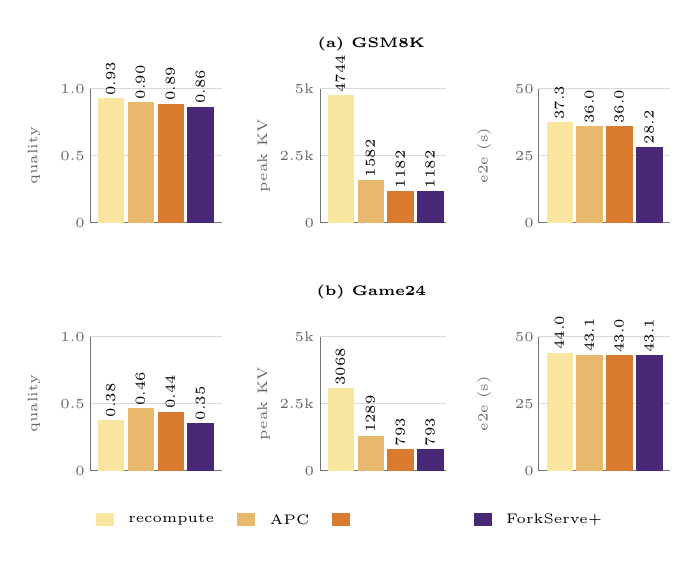
\begin{tikzpicture}[
  font=\scriptsize\sffamily,
  bar/.style={draw=black!55, line width=0.2pt},
  ax/.style={black!55, line width=0.35pt},
  grid/.style={black!15, line width=0.25pt},
  tick/.style={font=\tiny, text=black!60, inner sep=0pt},
  val/.style={font=\tiny, inner sep=0.3pt},
]
\definecolor{Rec}{HTML}{F8E6A0}
\definecolor{APC}{HTML}{E8B86D}
\definecolor{FS}{HTML}{D97B2F}
\definecolor{FSp}{HTML}{4A2878}

% --- (a) GSM8K, y shift 3.15 ---
\begin{scope}[shift={(0,3.15)}]
  \node[font=\tiny\bfseries] at (4.05,2.55) {(a) GSM8K};
  % quality, ymax 1.0
  \begin{scope}[shift={(0,0)}]
    \draw[grid] (0.48,0.28) -- (2.15,0.28) (0.48,1.13) -- (2.15,1.13) (0.48,1.98) -- (2.15,1.98);
    \draw[ax] (0.48,0.28) -- (2.15,0.28) (0.48,0.28) -- (0.48,1.98);
    \node[tick, anchor=east] at (0.42,0.28) {0};
    \node[tick, anchor=east] at (0.42,1.13) {0.5};
    \node[tick, anchor=east] at (0.42,1.98) {1.0};
    \node[tick, rotate=90, anchor=south] at (-0.15,1.13) {quality};
    \fill[bar, Rec] (0.58,0.28) rectangle (0.90,1.853);
    \fill[bar, APC] (0.96,0.28) rectangle (1.28,1.810);
    \fill[bar, FS]  (1.34,0.28) rectangle (1.66,1.788);
    \fill[bar, FSp] (1.72,0.28) rectangle (2.04,1.747);
    \node[val, rotate=90, anchor=west] at (0.74,1.87) {0.93};
    \node[val, rotate=90, anchor=west] at (1.12,1.83) {0.90};
    \node[val, rotate=90, anchor=west] at (1.50,1.81) {0.89};
    \node[val, rotate=90, anchor=west] at (1.88,1.77) {0.86};
  \end{scope}
  % peak KV, ymax 5k
  \begin{scope}[shift={(2.85,0)}]
    \draw[grid] (0.55,0.28) -- (2.15,0.28) (0.55,1.13) -- (2.15,1.13) (0.55,1.98) -- (2.15,1.98);
    \draw[ax] (0.55,0.28) -- (2.15,0.28) (0.55,0.28) -- (0.55,1.98);
    \node[tick, anchor=east] at (0.48,0.28) {0};
    \node[tick, anchor=east] at (0.48,1.13) {2.5k};
    \node[tick, anchor=east] at (0.48,1.98) {5k};
    \node[tick, rotate=90, anchor=south] at (-0.08,1.13) {peak KV};
    \fill[bar, Rec] (0.65,0.28) rectangle (0.97,1.893);
    \fill[bar, APC] (1.03,0.28) rectangle (1.35,0.818);
    \fill[bar, FS]  (1.41,0.28) rectangle (1.73,0.682);
    \fill[bar, FSp] (1.79,0.28) rectangle (2.11,0.682);
    \node[val, rotate=90, anchor=west] at (0.81,1.91) {4744};
    \node[val, rotate=90, anchor=west] at (1.19,0.84) {1582};
    \node[val, rotate=90, anchor=west] at (1.57,0.70) {1182};
    \node[val, rotate=90, anchor=west] at (1.95,0.70) {1182};
  \end{scope}
  % e2e seconds, ymax 50, shorter is faster
  \begin{scope}[shift={(5.70,0)}]
    \draw[grid] (0.48,0.28) -- (2.15,0.28) (0.48,1.13) -- (2.15,1.13) (0.48,1.98) -- (2.15,1.98);
    \draw[ax] (0.48,0.28) -- (2.15,0.28) (0.48,0.28) -- (0.48,1.98);
    \node[tick, anchor=east] at (0.42,0.28) {0};
    \node[tick, anchor=east] at (0.42,1.13) {25};
    \node[tick, anchor=east] at (0.42,1.98) {50};
    \node[tick, rotate=90, anchor=south] at (-0.12,1.13) {e2e (s)};
    \fill[bar, Rec] (0.58,0.28) rectangle (0.90,1.550);
    \fill[bar, APC] (0.96,0.28) rectangle (1.28,1.504);
    \fill[bar, FS]  (1.34,0.28) rectangle (1.66,1.505);
    \fill[bar, FSp] (1.72,0.28) rectangle (2.04,1.239);
    \node[val, rotate=90, anchor=west] at (0.74,1.57) {37.3};
    \node[val, rotate=90, anchor=west] at (1.12,1.52) {36.0};
    \node[val, rotate=90, anchor=west] at (1.50,1.52) {36.0};
    \node[val, rotate=90, anchor=west] at (1.88,1.26) {28.2};
  \end{scope}
\end{scope}

% --- (b) Game24 ---
\begin{scope}[shift={(0,0)}]
  \node[font=\tiny\bfseries] at (4.05,2.55) {(b) Game24};
  \begin{scope}[shift={(0,0)}]
    \draw[grid] (0.48,0.28) -- (2.15,0.28) (0.48,1.13) -- (2.15,1.13) (0.48,1.98) -- (2.15,1.98);
    \draw[ax] (0.48,0.28) -- (2.15,0.28) (0.48,0.28) -- (0.48,1.98);
    \node[tick, anchor=east] at (0.42,0.28) {0};
    \node[tick, anchor=east] at (0.42,1.13) {0.5};
    \node[tick, anchor=east] at (0.42,1.98) {1.0};
    \node[tick, rotate=90, anchor=south] at (-0.15,1.13) {quality};
    \fill[bar, Rec] (0.58,0.28) rectangle (0.90,0.917);
    \fill[bar, APC] (0.96,0.28) rectangle (1.28,1.067);
    \fill[bar, FS]  (1.34,0.28) rectangle (1.66,1.025);
    \fill[bar, FSp] (1.72,0.28) rectangle (2.04,0.875);
    \node[val, rotate=90, anchor=west] at (0.74,0.94) {0.38};
    \node[val, rotate=90, anchor=west] at (1.12,1.09) {0.46};
    \node[val, rotate=90, anchor=west] at (1.50,1.05) {0.44};
    \node[val, rotate=90, anchor=west] at (1.88,0.90) {0.35};
  \end{scope}
  \begin{scope}[shift={(2.85,0)}]
    \draw[grid] (0.55,0.28) -- (2.15,0.28) (0.55,1.13) -- (2.15,1.13) (0.55,1.98) -- (2.15,1.98);
    \draw[ax] (0.55,0.28) -- (2.15,0.28) (0.55,0.28) -- (0.55,1.98);
    \node[tick, anchor=east] at (0.48,0.28) {0};
    \node[tick, anchor=east] at (0.48,1.13) {2.5k};
    \node[tick, anchor=east] at (0.48,1.98) {5k};
    \node[tick, rotate=90, anchor=south] at (-0.08,1.13) {peak KV};
    \fill[bar, Rec] (0.65,0.28) rectangle (0.97,1.323);
    \fill[bar, APC] (1.03,0.28) rectangle (1.35,0.718);
    \fill[bar, FS]  (1.41,0.28) rectangle (1.73,0.550);
    \fill[bar, FSp] (1.79,0.28) rectangle (2.11,0.550);
    \node[val, rotate=90, anchor=west] at (0.81,1.34) {3068};
    \node[val, rotate=90, anchor=west] at (1.19,0.74) {1289};
    \node[val, rotate=90, anchor=west] at (1.57,0.57) {793};
    \node[val, rotate=90, anchor=west] at (1.95,0.57) {793};
  \end{scope}
  \begin{scope}[shift={(5.70,0)}]
    \draw[grid] (0.48,0.28) -- (2.15,0.28) (0.48,1.13) -- (2.15,1.13) (0.48,1.98) -- (2.15,1.98);
    \draw[ax] (0.48,0.28) -- (2.15,0.28) (0.48,0.28) -- (0.48,1.98);
    \node[tick, anchor=east] at (0.42,0.28) {0};
    \node[tick, anchor=east] at (0.42,1.13) {25};
    \node[tick, anchor=east] at (0.42,1.98) {50};
    \node[tick, rotate=90, anchor=south] at (-0.12,1.13) {e2e (s)};
    \fill[bar, Rec] (0.58,0.28) rectangle (0.90,1.775);
    \fill[bar, APC] (0.96,0.28) rectangle (1.28,1.747);
    \fill[bar, FS]  (1.34,0.28) rectangle (1.66,1.741);
    \fill[bar, FSp] (1.72,0.28) rectangle (2.04,1.744);
    \node[val, rotate=90, anchor=west] at (0.74,1.80) {44.0};
    \node[val, rotate=90, anchor=west] at (1.12,1.77) {43.1};
    \node[val, rotate=90, anchor=west] at (1.50,1.76) {43.0};
    \node[val, rotate=90, anchor=west] at (1.88,1.76) {43.1};
  \end{scope}
\end{scope}

\fill[Rec] (0.55,-0.42) rectangle (0.78,-0.26);
\node[font=\tiny, anchor=west] at (0.84,-0.34) {recompute};
\fill[APC] (2.35,-0.42) rectangle (2.58,-0.26);
\node[font=\tiny, anchor=west] at (2.64,-0.34) {APC};
\fill[FS] (3.55,-0.42) rectangle (3.78,-0.26);
\node[font=\tiny, anchor=west] at (3.84,-0.34) {\sys};
\fill[FSp] (5.35,-0.42) rectangle (5.58,-0.26);
\node[font=\tiny, anchor=west] at (5.64,-0.34) {ForkServe+};
\end{tikzpicture}
